\documentclass[12pt,a4paper]{article}

% Packages
\usepackage[utf8]{inputenc}
\usepackage[T1]{fontenc}
\usepackage{lmodern}
\usepackage{geometry}
\usepackage{graphicx} 
\usepackage{listings} 
\usepackage{xcolor} 
\usepackage{hyperref} 
\usepackage{amsmath, amssymb} 
\usepackage{caption} 
\usepackage{appendix}
\usepackage{enumitem}
% Page setup
\geometry{
 a4paper,
 left=25mm,
 right=25mm,
 top=25mm,
 bottom=25mm
}

% Code style
\lstset{
    basicstyle=\ttfamily\small,
    backgroundcolor=\color{gray!10},
    frame=single,
    breaklines=true,
    postbreak=\mbox{\textcolor{red}{$\hookrightarrow$}\space},
    numbers=left,
    numberstyle=\tiny,
    stepnumber=1,
    numbersep=5pt
}

% Title
\title{\vspace{-2cm}Assignment 1: Data Extraction \& Integration}
\author{Leonardo Rossi \\ Alice Bianchi \\ Marco Verdi} % replace with your names
\date{\today}

\begin{document}

\maketitle
\thispagestyle{empty}

\tableofcontents
\newpage

\section{Introduction}
As we read the tasks and rack our brains to redesign the dataset, we realised something important. Data Managers build the dataset according to the business; therefore, we should do likewise with our trading company. We assumed we are a B2B trading company in the IT industry. Our partners, such as NVIDIA and AMD, provides us the GPU and CPU at discounted price, that we resell in EU market. 
% \subsection{Tasks}
% To facilitate the reading, we added hypertext connectors from the tasks below to our answers:\\\\
% \textbf{Task 1: Database (re)design}
% \begin{enumerate}[label=(\alph*)]
%     \item \hyperref[sec:task1a]{Add more attributes to the given relations (bill, customer, partner).}
%     \item \hyperref[sec:task1b]{Add a minimum of two relations that represent entities. Make sure that there is at least one many-to-many relationship between the entities.}
%     \item \hyperref[sec:task1c]{Draw the schema chart for the database.}
%     \item \hyperref[sec:task1d]{Identify the cardinalities of the relationships between the entities and explain how you can represent the relationships in your design.}
%     \item \hyperref[sec:task1e]{List all the primary-key-foreign-key constraints in the database.}
%     \item \hyperref[sec:task1f]{Write the SQL code that creates the whole database in SQLite and save the file as .sql.}
%     \item \hyperref[sec:task1g]{Pick one of the relations (tables) and explain if it is in the BCNF or not (justify your answer).}
% \end{enumerate}
% \textbf{Task 2: Querying the database}
% \begin{enumerate}[label=(\alph*)]
%     \item \hyperref[sec:task2a]{Joining more than two tables.}
%     \item \hyperref[sec:task2b]{Aggregate function.}
%     \item \hyperref[sec:task2c]{Nested query.}
% \end{enumerate}
% \textbf{Task 3: Data extraction and entity resolution using Python}
% \begin{enumerate}[label=(\alph*)]
%     \item \hyperref[sec:task3a]{Write a Python code that allows you to connect to the database file, send SQL queries to the database and extract the results.}
%     \item \hyperref[sec:task3b]{Read the content of the customer relation (table) into Pandas DataFrame.}
%     \item \hyperref[sec:task3c]{Using a similarity function that compares two records, report the customers with similarity $> 0.7$.}
% \end{enumerate}
\section{Task 1: Database (Re)design}
The database contains the following tables and relationships:

\begin{itemize}
    \item \textbf{bill}
    \begin{itemize}
        \item \textbf{Description:} This table stores the main features of each bill.
        \item \textbf{Columns:} \texttt{bill\_id}, \texttt{wh\_branch\_id}, \texttt{customer\_id}, \texttt{date}, \texttt{amount}, \texttt{payment\_method}.
        \item \textbf{Primary Key:} \texttt{bill\_id}.
        \item \textbf{Foreign Keys:} 
        \begin{itemize}
            \item \texttt{wh\_branch\_id} $\to$ \texttt{branch(branch\_id)}.
            \item \texttt{customer\_id} $\to$ \texttt{customer(customer\_id)}.
        \end{itemize}
        \item \textbf{Cardinality:}
        \begin{itemize}
             \item \textbf{(1:N)}: Each \texttt{bill} is linked to exactly one \texttt{branch} and one \texttt{customer}, while each \texttt{branch} and \texttt{customer} can be associated with multiple \texttt{bill\_id}s.
        \end{itemize}
    \end{itemize}

    \item \textbf{ref\_employees}
    \begin{itemize}
        \item \textbf{Description:} This table links each bill to the employee (e.g. salesman) who handled the deal and, optionally, to the purchasing contact from the client side. It allows tracking employee performance and customer interactions.
        \item \textbf{Columns:} \texttt{bill\_id}, \texttt{ref\_employee\_id}, \texttt{ref\_cust\_id}.
        \item \textbf{Primary Key:} \texttt{bill\_id}.
        \item \textbf{Foreign Keys:} 
        \begin{itemize}
            \item \texttt{bill\_id} $\to$ \texttt{bill(bill\_id)}.
            \item \texttt{ref\_employee\_id} $\to$ \texttt{employees(employee\_id)}.
            \item \texttt{ref\_cust\_id} $\to$ \texttt{ref\_customers(reference\_id)}.
        \end{itemize}
        \item \textbf{Cardinality:}
        \begin{itemize}
             \item \textbf{(1:1)}: Each \texttt{ref\_employees} entry corresponds to exactly one \texttt{bill}.
             \item \textbf{(1:N)}: Each \texttt{employee} can be linked to multiple bills.
             \item \textbf{(0:N)}: Each \texttt{ref\_cust\_id} can be NULL, but when exist, one contact can be associated with multiple bills.
        \end{itemize}
    \end{itemize}

    \item \textbf{country\_tbl}
    \begin{itemize}
        \item \textbf{Description:} This table stores information about countries, code, name, and international phone code.
        \item \textbf{Columns:} \texttt{country}, \texttt{country\_name}, \texttt{country\_phone\_code}.
        \item \textbf{Primary Key:} \texttt{country}.
        \item \textbf{Constraints:}
        \texttt{country\_name} and \texttt{country\_phone\_code} are both \texttt{UNIQUE} and cannot be \texttt{NULL}.

        \item \textbf{Cardinality:}
        \begin{itemize}
             \item \textbf{(1:1)}: Each country code corresponds to exactly one country name and one phone code.
        \end{itemize}
    \end{itemize}

    \item \textbf{sector\_tbl}
    \begin{itemize}
        \item \textbf{Description:} This table defines economic sectors, mapping a short sector code to a sector label and a descriptive explanation.
        \item \textbf{Columns:} \texttt{sector\_code}, \texttt{sector}, \texttt{sector\_desc}.
        \item \textbf{Primary Key:} \texttt{sector\_code}.
        \item \textbf{Constraints:}
             \texttt{sector} and \texttt{sector\_desc} are both \texttt{UNIQUE} and cannot be \texttt{NULL}.
        \item \textbf{Cardinality:}
        \begin{itemize}
             \item \textbf{(1:1)}: Each sector code corresponds to exactly one sector name and one description.
        \end{itemize}
    \end{itemize}

    \item \textbf{branch}
    \begin{itemize}
        \item \textbf{Description:} This table stores information about company branches, including their identifier, name, location (city), and the country in which they are located.
        \item \textbf{Columns:} \texttt{branch\_id}, \texttt{name}, \texttt{city}, \texttt{country}.
        \item \textbf{Primary Key:} \texttt{branch\_id}.
        \item \textbf{Foreign Keys:} 
        \begin{itemize}
            \item \texttt{country} $\to$ \texttt{country\_tbl(country)}.
        \end{itemize}
        \item \textbf{Cardinality:}
        \begin{itemize}
             \item \textbf{(1:N)}: Each \texttt{branch} belongs to exactly one \texttt{country}, while each \texttt{country} can be linked to multiple \texttt{branches}.
        \end{itemize}
    \end{itemize}

\item \textbf{customer}
    \begin{itemize}
        \item \textbf{Description:} Stores customer company information, including identifiers, sector, address, and country.
        \item \textbf{Columns:} \texttt{customer\_id}, \texttt{company\_name}, \texttt{sector\_code}, \texttt{country}, \texttt{street}, \texttt{house\_number}, \texttt{zip\_code}, \texttt{city}.
        \item \textbf{Primary Key:} \texttt{customer\_id}.
        \item \textbf{Foreign Keys:}
        \begin{itemize}
            \item \texttt{sector\_code} $\to$ \texttt{sector\_tbl(sector\_code)}.
            \item \texttt{country} $\to$ \texttt{country\_tbl(country)}.
        \end{itemize}
        \item \textbf{Cardinality:}
        \begin{itemize}
            \item \textbf{(1:N)}: Each \texttt{sector} and \texttt{country} can be linked to multiple \texttt{customers}.
        \end{itemize}
    \end{itemize}

    \item \textbf{ref\_customers}
    \begin{itemize}
        \item \textbf{Description:} Stores individual references/contacts of customers with their personal and professional info.
        \item \textbf{Columns:} \texttt{reference\_id}, \texttt{customer\_id}, \texttt{name}, \texttt{surname}, \texttt{role}, \texttt{email}, \texttt{country}, \texttt{country\_phone\_code}, \texttt{phone\_number}.
        \item \textbf{Primary Key:} \texttt{reference\_id}.
        \item \textbf{Foreign Keys:}
        \begin{itemize}
            \item \texttt{customer\_id} $\to$ \texttt{customer(customer\_id)}
             \item (\texttt{country}, \texttt{country\_phone\_code}) $\to$ \texttt{country\_tbl(country, country\_phone\_code)}
        \end{itemize}
        \item \textbf{Cardinality:}
        \begin{itemize}
            \item \textbf{(1:N)}: Each \texttt{customer} (company) and \texttt{country} can have multiple \texttt{references} (employees), while each \texttt{reference} can have only one\texttt{customer}.
             \item \textbf{(1:N)}: Each \texttt{country} (and phone code) can be linked to multiple \texttt{references}.
        \end{itemize}
      \end{itemize}  
  \item \textbf{partner}
    \begin{itemize}
        \item \textbf{Description:} Stores information on partner companies, their sector, country, and contact details.
        \item \textbf{Columns:} \texttt{partner\_id}, \texttt{company\_name}, \texttt{country}, \texttt{products\_and\_services}, \texttt{sector\_code}, \texttt{contact\_person}, \texttt{contact\_email}.
        \item \textbf{Primary Key:} \texttt{partner\_id}.
        \item \textbf{Foreign Keys:}
        \begin{itemize}
            \item \texttt{country} $\to$ \texttt{country\_tbl(country)} \\
            \hspace{1cm} \textit{ON UPDATE CASCADE}.
            \item \texttt{sector\_code} $\to$ \texttt{sector\_tbl(sector\_code)} \\
            \hspace{1cm} \textit{ON UPDATE CASCADE}.
        \end{itemize}
        \item \textbf{Cardinality:}
        \begin{itemize}
            \item \textbf{(1:N)}: Each country can host multiple partners.
            \item \textbf{(1:N)}: Each sector can be associated with multiple partners.
        \end{itemize}
    \end{itemize}

     \item \textbf{employees}
    \begin{itemize}
        \item \textbf{Description:} Stores information on employees working in branches, including contact details and organisational role.
        \item \textbf{Columns:} \texttt{employee\_id}, \texttt{branch\_id}, \texttt{name}, \texttt{surname}, \texttt{role}, \texttt{department}, \texttt{email}, \texttt{phone\_number}.
        \item \textbf{Primary Key:} \texttt{employee\_id}.
        \item \textbf{Foreign Keys:}
        \begin{itemize}
            \item \texttt{branch\_id} $\to$ \texttt{branch(branch\_id)} \\
            \hspace{1cm} \textit{ON UPDATE CASCADE, ON DELETE CASCADE}.
        \end{itemize}
        \item \textbf{Cardinality:} \textbf{(1:N)}: Each branch can employ multiple employees, while each employee belongs to exactly one branch.
    \end{itemize}


   \item \textbf{items}
    \begin{itemize}
        \item \textbf{Description:} Stores information on items sold, including their technical name, supplier, and purchase price.
        \item \textbf{Columns:} \texttt{item\_id}, \texttt{tech\_name}, \texttt{partner\_id}, \texttt{buy\_price}.
        \item \textbf{Primary Key:} \texttt{item\_id}.
        \item \textbf{Foreign Keys:}
        \begin{itemize}
            \item \texttt{partner\_id} $\to$ \texttt{partner(partner\_id)} \\
            \hspace{1cm} \textit{ON UPDATE CASCADE, ON DELETE SET NULL}.
        \end{itemize}
        \item \textbf{Cardinality:} \textbf{(1:N)}: Each partner can supply multiple items, while each item is supplied by at most one partner.
    \end{itemize}
        \item \textbf{status}
    \begin{itemize}
        \item \textbf{Description:} Tracks the evolution of a bill over time, including item status, payment status, and refund requests.
        \item \textbf{Columns:} \texttt{bill\_id}, \texttt{update\_date}, \texttt{status\_items}, \texttt{status\_payment}, \texttt{refund\_request}.
        \item \textbf{Primary Key:} Composite: \texttt{(bill\_id, update\_date)}.
        \item \textbf{Foreign Keys:} 
        \begin{itemize}
            \item \texttt{bill\_id} $\to$ \texttt{bill(bill\_id)} \\
            \hspace{1cm} \textit{ON UPDATE CASCADE, ON DELETE CASCADE}.
        \end{itemize}
        \item \textbf{Cardinality:}
        \begin{itemize}
            \item \textbf{(1:N)}: Each bill can have multiple status updates over time, while each status update belongs to exactly one bill.
        \end{itemize}
    \end{itemize}

    \item \textbf{bill\_item}
    \begin{itemize}
        \item \textbf{Description:} Stores the items sold in each bill, including quantity and price.
        \item \textbf{Columns:} \texttt{bill\_id}, \texttt{item\_id}, \texttt{quantity}, \texttt{price}.
        \item \textbf{Primary Key:} Composite: \texttt{(bill\_id, item\_id)}.
        \item \textbf{Foreign Keys:} 
        \begin{itemize}
            \item \texttt{bill\_id} $\to$ \texttt{bill(bill\_id)} \\
            \hspace{1cm} \textit{ON UPDATE CASCADE, ON DELETE CASCADE}.
            \item \texttt{item\_id} $\to$ \texttt{items(item\_id)} \\
            \hspace{1cm} \textit{ON UPDATE CASCADE}.
        \end{itemize}
        \item \textbf{Cardinality:}
        \begin{itemize}
            \item \textbf{(1:N)}: Each bill can contain multiple items, while each item can appear in multiple bills (\textbf{many-to-many} relationship).
        \end{itemize}
    \end{itemize}


    
\end{itemize}






\subsection{Normalization Analysis}
Explain if a table is in BCNF and justify your answer.

\section{Task 2: Querying the Database}
Describe your queries in natural language and relational algebra here.

\section{Task 3: Data Extraction and Entity Resolution Using Python}
Describe your Python approach, connection to the database, and similarity logic.

\section{Resources / Repository}
The full code, database files, and supplementary materials are available in our GitHub repository:  
\href{https://github.com/YourUsername/YourRepo}{https://github.com/YourUsername/YourRepo}

\newpage
\appendix
\section{Appendix A: Database Schema}
\begin{figure}[h!]
    \centering
    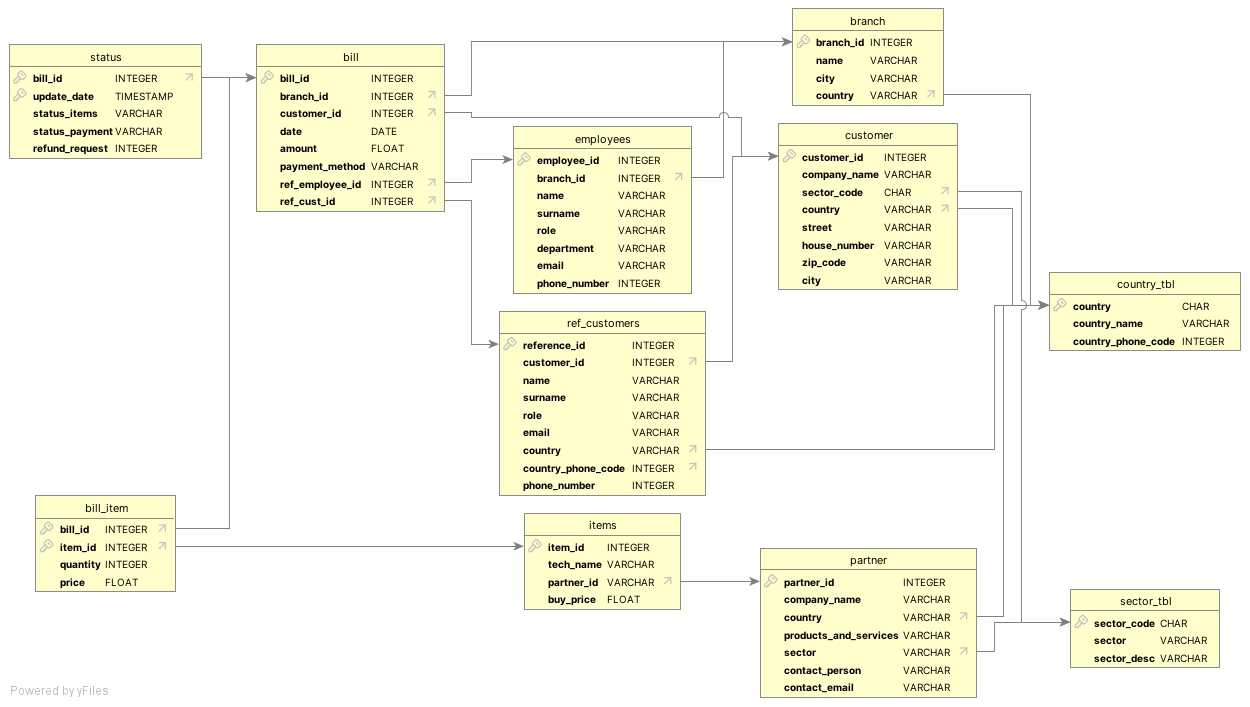
\includegraphics[width=1.1\textwidth]{ERdiagram.jpg} % replace with your schema image
    \caption{Database schema with relationships and cardinalities.}
    \label{fig:schema}
\end{figure}

\section{Appendix B: SQL Code}
\begin{lstlisting}[language=SQL]
-- Example: Create table
CREATE TABLE customer (
    customer_id INTEGER PRIMARY KEY,
    name TEXT,
    street TEXT,
    city TEXT,
    country TEXT
);
\end{lstlisting}

\section{Appendix C: Python Code}
\begin{lstlisting}[language=Python]
import sqlite3
import pandas as pd

conn = sqlite3.connect('database.db')
df = pd.read_sql_query("SELECT * FROM customer", conn)
print(df.head())
\end{lstlisting}

\end{document}
